\documentclass[crop, tikz]{standalone}
\usepackage{tikz}

\usetikzlibrary{decorations.pathmorphing}

\definecolor{bluport}{HTML}{21ADFD}
\definecolor{orgport}{HTML}{E37322}
\definecolor{pplport}{HTML}{4F21E9}
\definecolor{redport}{HTML}{701315}

\begin{document}
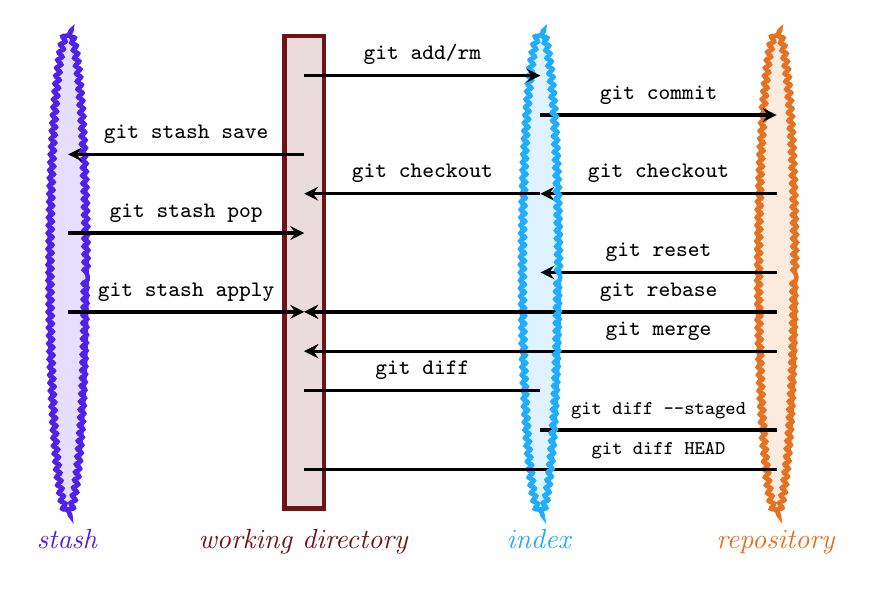
\begin{tikzpicture}

	\fill[pplport!15] (0, 0) ellipse (0.25 and 3);
	\fill[redport!15] (2.75, -3) rectangle (3.25, 3);
	\fill[bluport!15] (6, 0) ellipse (0.25 and 3);
	\fill[orgport!15] (9, 0) ellipse (0.25 and 3);
	
	\draw[thick, pplport] (0, 0) ellipse (0.25 and 3);
	\draw[ultra thick, pplport, decorate, decoration={snake, segment length=1mm, amplitude=0.3mm}] (0, 0) ellipse (0.23 and 3.05);
	\node[text height=1em, text depth=1em, pplport] (1) at (0, -3.5) {\emph{stash}};
		
	\draw[ultra thick, redport] (2.75, -3) rectangle (3.25, 3);
	\node[text height=1em, text depth=1em, redport] (2) at (3, -3.5) {\emph{working directory}};
		
	\draw[thick, orgport] (9, 0) ellipse (0.25 and 3);
	\draw[ultra thick, orgport, decorate, decoration={snake, segment length=1mm, amplitude=0.3mm}] (9, 0) ellipse (0.23 and 3.05);
	\node[text height=1em, text depth=1em, orgport] (4) at (9, -3.5) {\emph{repository}};
	
	\draw[-stealth, very thick] (6, 2) -- node[above] {\tt\footnotesize git commit} (9, 2);
	\draw[-stealth, very thick] (9, 1) -- node[above] {\tt\footnotesize git checkout} (6, 1);
	\draw[-stealth, very thick] (9, 0) -- node[above] {\tt\footnotesize git reset} (6, 0);
	\draw[very thick] (6, -2) -- node[above] {\tt\scriptsize git diff -{}-staged} (9, -2);
	\draw[very thick] (3, -2.5) -- node[above, pos=0.75] {\tt\scriptsize git diff HEAD} (9, -2.5);
	\draw[-stealth, very thick] (9, -0.5) -- node[above, pos=0.25] {\tt\footnotesize git rebase} (3, -0.5);
	\draw[-stealth, very thick] (9, -1) -- node[above, pos=0.25] {\tt\footnotesize git merge} (3, -1);
	
	% draw the blue portal here for the portal effect
	\draw[thick, bluport] (6, 0) ellipse (0.25 and 3);
	\draw[ultra thick, bluport, decorate, decoration={snake, segment length=1mm, amplitude=0.3mm}] (6, 0) ellipse (0.23 and 3.05);
	\node[text height=1em, text depth=1em, bluport] (3) at (6, -3.5) {\emph{index}};
	
	% Redraw some lines for piercing effect through blu port
	\draw[-stealth, very thick] (6, -0.5) -- (3, -0.5);
	\draw[-stealth, very thick] (6, -1) -- (3, -1);	
	\draw[very thick] (3, -2.5) -- (6, -2.5);
	
	\draw[-stealth, very thick] (3, 2.5) -- node[above] {\tt\footnotesize git add/rm} (6, 2.5);
	\draw[-stealth, very thick] (3, 1.5) -- node[above] {\tt\footnotesize git stash save} (0, 1.5);
	\draw[-stealth, very thick] (6, 1) -- node[above] {\tt\footnotesize git checkout} (3, 1);
	\draw[-stealth, very thick] (0, 0.5) -- node[above] {\tt\footnotesize git stash pop} (3, 0.5);
	\draw[-stealth, very thick] (0, -0.5) -- node[above] {\tt\footnotesize git stash apply} (3, -0.5);
	\draw[very thick] (3, -1.5) -- node[above] {\tt\footnotesize git diff} (6, -1.5);
\end{tikzpicture}
\end{document}
